\chapter{Grobkonzept und technische Grundlagen}
\label{TechnischeGrundlagen}
In diesem Kapitel wird erst das Grobkonzept des Longboards Commute von Skatemate dargestellt, um einen Überblick über das Elektroskateboard zu geben.
Anschliessend werden die notwendigen technischen Grundlagen erklärt, so dass die Hardware und Software besser verstanden werden können.
\todo{bessere Einleitung / ... anpassen}

\todo{Ziel - Aufgabe - Anforderung pro Unterkapitel oder pro ... kA was}

\section{Grobkonzept}
\label{Grobkonzept}
\todo{Einstieg, beginnt zu sehr im Detail...?}

Das Projekt Commute von Skatemate kann in drei Grundbereiche unterteilt werden: Die innovative Steuerung, die Motorregelung und die Stromversorgung. 
In den folgenden Unterkapitel werden diese drei Bereiche und die dazugehörigen Begriffe detaillierter erläutert. Die intuitive Bedienung des Longboards geschieht über eine Fingerbewegung, welche dank des Magic Gloves gemessen werden kann. Der Motor wird mithilfe der Feldorientierten Regelung FOC angesteuert, mit dieser Regelungstechnik können Wechselgrössen elegant gesteuert werden. Die Stromversorgung verfügt über ein eigens dazu konzipiertes Akkuladegerät. 
\begin{figure}[H]
	\centering
	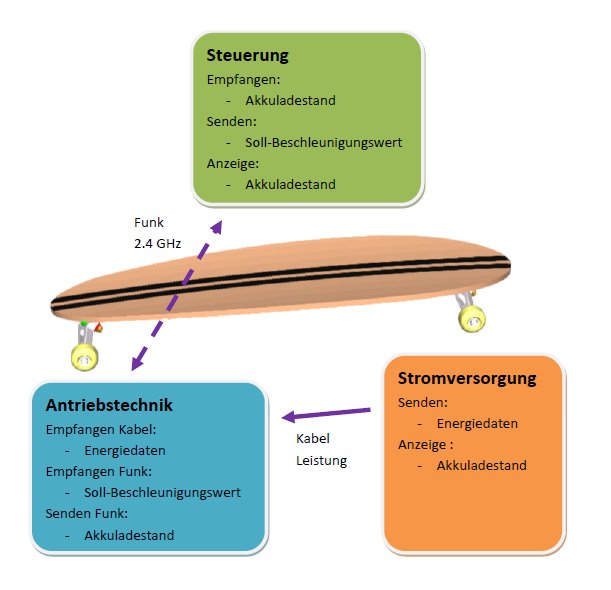
\includegraphics[width=0.8\linewidth, keepaspectratio]{images/Grobkonzept_Blockschaltbild_grob}
	\caption[Blockschaltbild Grobkonzept]{Blockschaltbild Grobkonzept}
	\label{fig:grobkonzeptblockschaltbildgrob}
\end{figure}
Wie sie miteinander interagieren, ist in der Abbildung \ref{fig:grobkonzeptblockschaltbildgrob} dargestellt. Die Antriebstechnik ist über ein Kabel mit der Stromversorgung verbunden, die Inputs der Steuerung erhält sie über ein Funknetz. \\
Um eine Übersicht über die enthaltenen Komponenten der drei genannten Bereiche zu erhalten, sind sie im Blockschaltbild der Abbildung \ref{fig:grobkonzeptblockschaltbilddetailliert} dargestellt.

 \todo{Zudem wird darauf eingegangen, weshalb diese Lösung gewählt wurde. }

\begin{figure}[h]
	\centering
	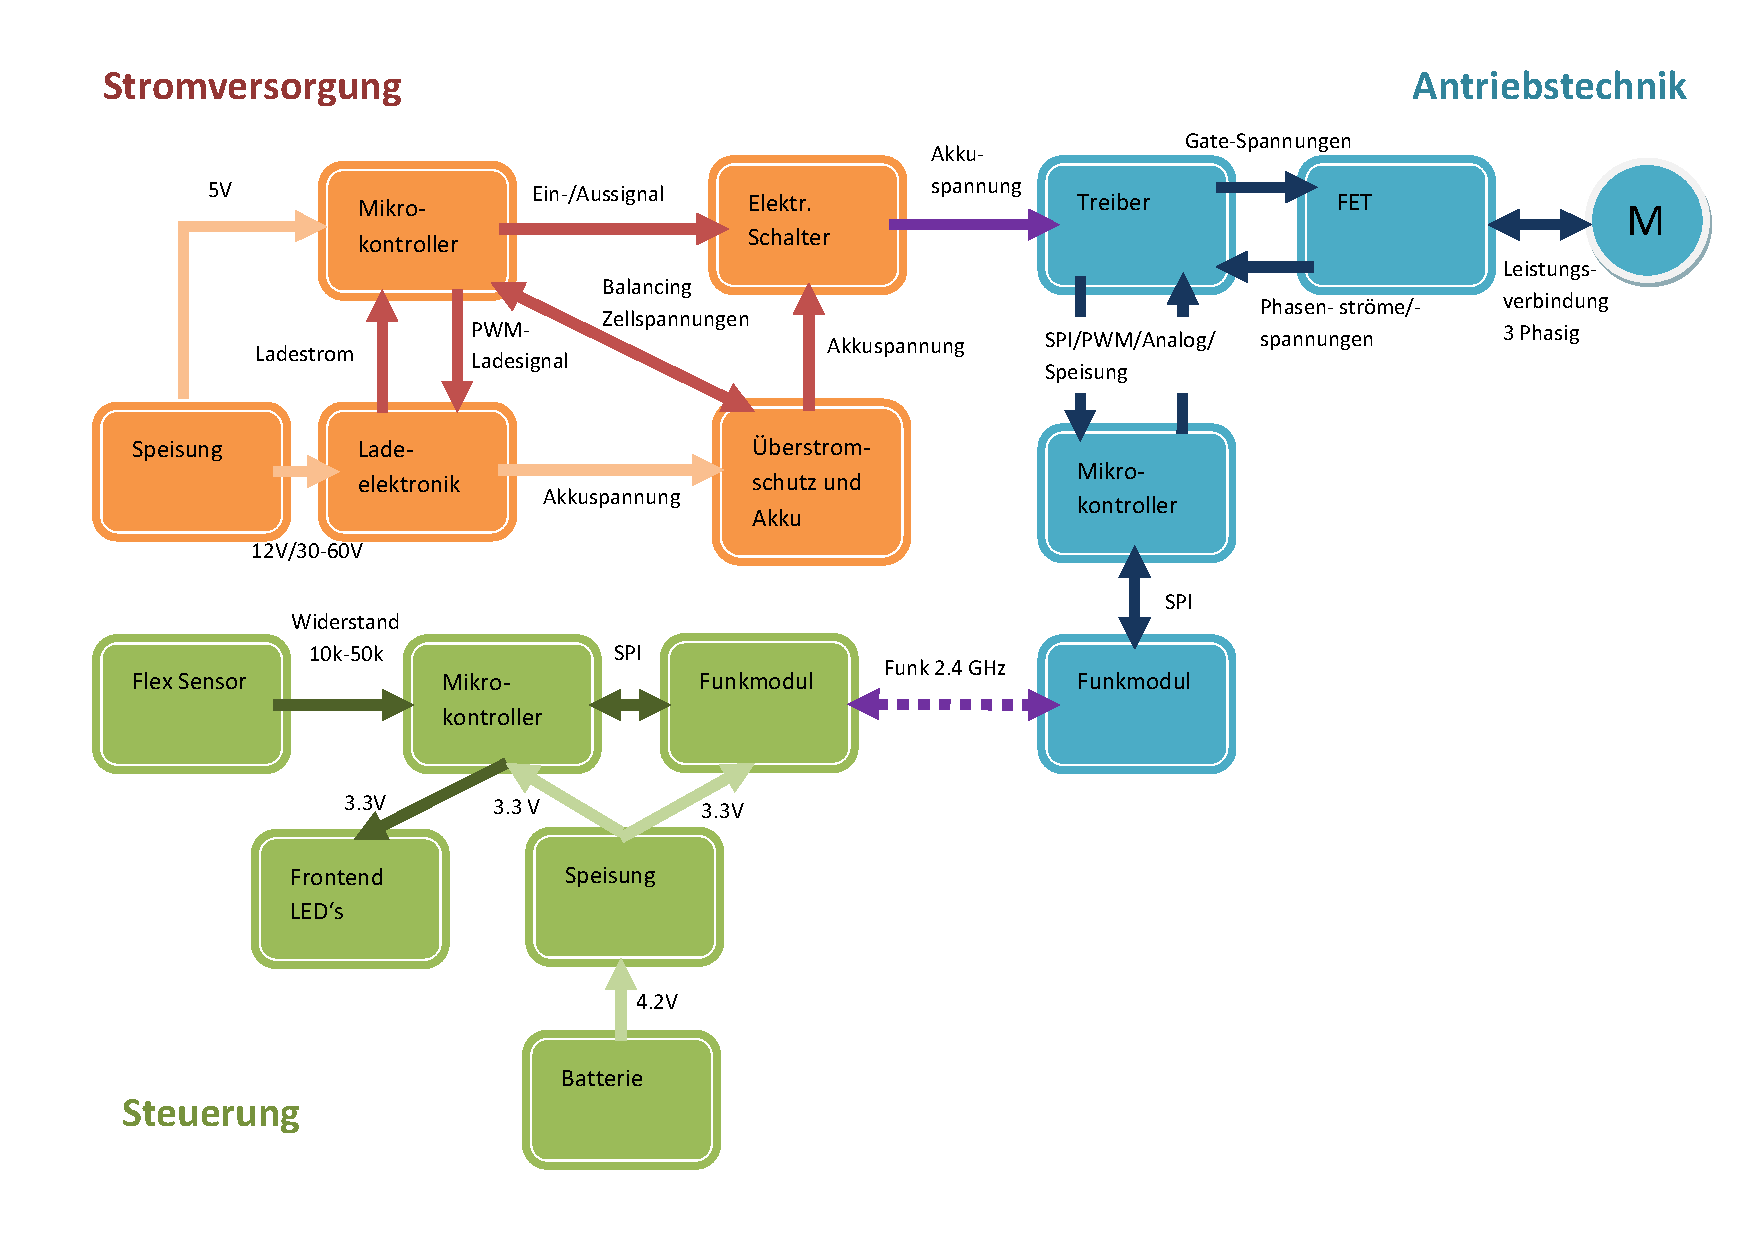
\includegraphics[width=\linewidth]{images/Grobkonzept_Blockschaltbild_detailliert}
	\caption[Detailliertes Blockschaltbild]{Detailliertes Blockschaltbild}
	\label{fig:grobkonzeptblockschaltbilddetailliert}
\end{figure}

\subsection*{Steuerung über den Magic Glove}
Es gibt verschiedene Wege, wie ein elektrisches Longboard gesteuert werden kann. Eine Variante ist, über Drucksensoren im Brett durch eine Gewichtsverlagerung in Fahrtrichtung eine Geschwindigkeitsregulation zu erreichen. Da auf unebenem Gelände das Gewicht laufend ausbalanciert werden muss, müssten diese Bewegungsimpulse kompensiert werden. Ausserdem können lokal begrenzte Sensoren die Bewegungsfreiheit auf dem Longboard einschränken.
Aus diesen Gründen wurde diese Variante verworfen. Das Team hat sich stattdessen entschieden, die Geschwindigkeit über eine Fingerbewegung zu steuern. Dazu wird ein Handschuh mit integrierten Sensoren entwickelt. Dieses Wearable enthält einen Flex Sensor, der die Beugung des Zeigefinders misst. Dieser Messvorgang und der Flex Sensor werden im Kapitel \ref{tGl_FlexSensor} beschrieben. Die mit dem Flex Sensor gemessene Beugung des Fingers wird mithilfe eines Mikrocontrollers quantifiziert. Diese Sollbeschleunigung wird anschliessend der Motoransteuerung übermittelt. Dies geschieht über ein 2.4 GHz-Funknetz, dazu ist ein Funkmodul integriert. Die Stromversorgung erfolgt über eine Li-Ion Knopfbatterie LTR2450. In der Abbildung \ref{fig:grobkonzeptblockschaltbilddetailliert} sind die genannten Elemente der Steuerung dargestellt.

\subsection*{Antriebstechnik}
\todo{def., Aufgabe ?}
Als Antrieb ist der OX1 2-10 Motor vorgegeben. Dies ist ein Bürstenloser-Gleichstrommotor (brushless DC motor, BLDC-Motor). Er verfügt nicht über Hallsensoren, mit denen die Rotorposition gemessen werden könnte. Die technischen Hintergründe des Motors werden im Kapitel \ref{tGl_BLDC} gegeben. Ein BLDC-Motor ist wie ein permanentmagnetischer Drehstrom-Synchronmotor (PMSM) aufgebaut.\\
Zur Ansteuerung gibt es grob unterteilt zwei verschiedene Arten, die Kommutierung und die Feldorientierte Regelung (FOC) \cite{BLDC}. \todo{[ Quelle xxx ]}. Die Kommutierung wiederum kann auf zwei verschiedene Arten erfolgen, ungesteuert (Blockkommutierung) oder gesteuert (Sinus-Kommutierung). Diese resultierenden drei Ansteuerungsmöglichkeiten sind in der Tabelle \ref{tabMotcontrVarProCon} zur Übersicht dargestellt und nachfolgend etwas genauer erläutert. 
\begin{center}
	\begin{tabularx}{\textwidth}{|c|X|X|}
		\hline 
		\textbf{Regelungsart} & \textbf{Vorteile} & \textbf{Nachteile} \\ 
		\hline 
		\textbf{Blockkommutierung} & einfach & schlechte Effizienz (eine Spule nicht gebraucht) 
		
		Drehmoment-Rippel \\
		\hline 
		\textbf{Sinus-Kommutierung} & alle drei Spulen benutzt & kompliziert
		
		Anfahren erschwert \\ 
		\hline 
		\textbf{FOC} & dynamisch 
		
		effizient 
		
		durch Trafo einfacher PI-Regler & Einstieg komplex \\ 
		\hline 
	\end{tabularx} 
	\captionof{table}{Vor- und Nachteile der verschiedenen Regelungsarten}
	\label{tabMotcontrVarProCon}
\end{center}

\todo{Tabelle formatieren!... ??}

Bei der ungesteuerten Kommutierung (Blockkommutierung) wird der Motor als Schrittmotor genutzt. Dabei folgt die Rotorposition der Steuerung. Diese Variante ist für ein gleichmässig rollendes Longboard ungeeignet, da der Schrittmotor nicht durchgehend sondern immer nur schrittweise dreht. Für ein gleichmässiges Drehen muss die Kommutierung also abhängig von der Rotorposition erfolgen (geführte Kommutierung, Sinus-Kommutierung). Dabei reagiert die Steuerung auf die effektive Rotorposition und passt sich dieser an.\todo{(xxx korrekt?} Am einfachsten wäre dies mit Sensoren, da der Motor jedoch nicht über Sensoren verfügt, muss der Motor über eine sensorlos gesteuerte Kommutierung angesteuert werden. Dies funktioniert jedoch nur ab einer Mindestdrehzahl wirklich gut. Zum Anfahren muss der Motor speziell angesteuert werden. \\
Bei der Feldorientierte Regelung (field oriented controll, FOC), werden die Spannungen zur Steuerung aktiv der Rotorlage angepasst. Dabei kann zwischen sensorgesteuerte und sensorlosen Regelung unterschieden werden. Bei der sensorlosen Regelung muss wiederum zum Anfahren eine zusätzliche Ansteuerung erfolgen. Kann die Anfangsposition ausreichend genau geschätzt werden, läuft der Motor auch bei tiefen Geschwindigkeiten gleichmässig, da er genauer geregelt werden kann. Dies entspricht unseren Anforderungen für das Commute, da ein sanftes Anfahren sehr wichtig ist. Die FOC als auch die Anfahr-Ansteuerung ist im Kapitel \ref{tGl_FOC} erklärt.\\
Ausgeführt wird die FOC auf einem Mikrocontroller. Mittels eines RF-Modul wird die Sollbeschleunigung empfangen. Eine Halbbrücke mit FET-Treibern (siehe Kapitel \ref{tGl_HBrugg}) setzt  die gewünschte Motorsteuerung um. Zur Übersicht sind diese Elemente im Blockschaltbild Abbildung \ref{fig:grobkonzeptblockschaltbilddetailliert} dargestellt. 

\subsection*{Stromversorgung}
Die Stromversorgung erfolgt über einen LiPo-5200mAh-Akku, dieser ist vorgegeben. Zwar besteht ein externes Ladegerät, doch dies bedeutet, dass der Akku für jedes Laden vom Longboard gelöst werden muss. Das ist umständlich und gefährdet die Wetterfestigkeit und Robustheit des Commute. Deshalb wird ein eigener, integrierter Akkulader entwickelt, so dass der Akku nicht mehr herausgelöst werden muss. Da die Entladung im Gebrauch sowieso überwacht werden muss, ist der Lader eine Ergänzung und kein alleinstehendes Element. Kernstück der Stromversorgung ist die Balancerschaltung. Dabei wird der Akku erst mit einem konstanten Strom geladen, bis die Zellspannung erreicht ist. Anschliessend wird mit einer konstanten Spannung geladen, bis der Strom unter 100mA gesunken ist, dann sind die Zellen vollständig geladen. Wie das Balancing genau funktioniert, ist im Kapitel \ref{tGl_Balancing} beschrieben. Anstelle einer eigenen Implementation hätte ein fertiges IC eingekauft werden können. Aus finanziellen Gründen wurde jedoch darauf verzichtet. Die Elemente der Stromversorgung sind in der Abbildung \ref{fig:grobkonzeptblockschaltbilddetailliert} dargestellt.

\todo{ev: wie viel Strom braucht der Motor? Wie weit reicht eine Akkuladung?}

%-----------------------------------------------------------------------------------------------------------------------------------------------------------------------------

\section{Technische Grundlagen}
In den folgenden Unterkapiteln werden die technischen Grundlagen zum Verständnis der Hard- und Software erläutert, so dass deren Funktionsweisen verstanden werden können.  
\subsection{Flex Sensor}
\label{tGl_FlexSensor}
Ein Flex Sensor eignet sich dazu, als analoges elektrisches Bauteil, eine Biegung zu messen. Im Falle dieses Projekts dazu zu erkennen wie fest der Finger des Fahrers gebogen ist. 
Der Sensor ändert je nach Biegung seinen Widerstandswert im Bereich von 13 bis ca. 80kOhm bei der stärksten Verformung. Das Bauteil selbst besteht aus einem flexiblen PCB mit einer
darauf befestigten Schicht von metallischen Partikeln. Wird der Sensor nun gebogen, entfernen sich die Partikel nun voneinander, vergrössert sich der Widerstand. Biegt man den Sensor
wiederum zurück in seine Ausgangsposition, verkleinert sich der Wiederstandswert wieder.

Um diesen Widerstand messen zu können wurde eine Verstärkerschaltung mit Messbrücke aufgebaut s.h. Abbildung 2.3 untenstehend. Der Widerstand der als Flex Sensor angeschrieben ist, verfügt über einen Wertebereich von 13 bis 80 Kiloohm. Mit den beiden Widerständen R2 und R3 wird die Untergrenze der Messbaren Resistanz festgelegt. Mit R1 wird schliesslich die Skalierung der Brücke festgelegt. Die resultierenden Spannungen zwischen R1 und R2 bzw. zwischen R3 und R4 werden schliesslich durch einen Rail-To-Rail Operationsverstärker so fest verstärkt, dass sie den Spannungsbereich von 0 bis 3.3 Volt ausnutzen. Dadurch kann schliesslich der
angehängte 10bit A/D-Wandler vollständig ausgesteuert werden.
\begin{figure} [H]
	\centering

\subfigure[Funktionsprinzip FlexSensor]{
	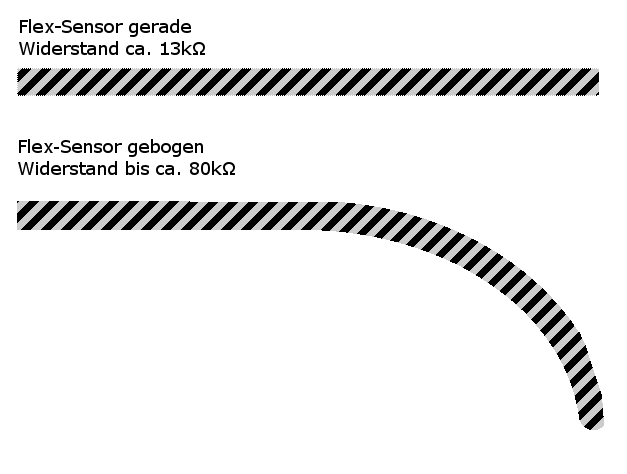
\includegraphics[width=0.45\linewidth]{images/FlexSensor} \label{FlexSensor} 	}
\subfigure[Sinstr][Messbrücke für FlexSensor]{ 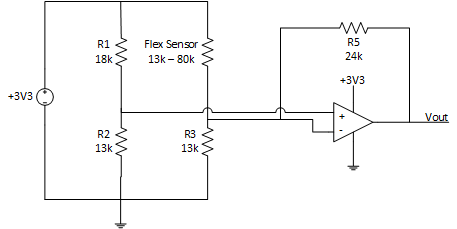
\includegraphics[width=0.5\linewidth]{images/FlexSensor_Messbruecke} \label{FlexSensor_Messbruecke}}
\caption[BLDC Motor]{Funktionsprinzip und Ansteuerung für einen FlexSensor}
\label{fig:BLDC}
\end{figure}
\subsection{Balancing}
\label{tGl_Balancing}
Das Board wird durch einen sechs Zellen Li-Po Akku gespeist. Jede einzelne Zelle hat dabei einen eigenen Innenwiderstand, welcher sich mit dem Alter verändern kann. Beim Ladevorgang entstehen somit unterschiedliche Spannungen wodurch die Zellen aus der Balance geraten.
Damit sich einzelne Zellen nicht überladen während andere leer bleiben, benötigt es einen Balancing-Vorgang um die Differenzen der Zellen auszugleichen. 
Dabei werden bei einer zu grossen Spannungsdifferenz alle Zellen auf die Spannung der niedrigsten Zelle entladen. Dabei wird in unserem Fall die überschüssige Energie über den Transistor und die Widerstände verheizt.

\subsection{BLDC Motor}
\label{tGl_BLDC}

Für dieses Projekt wurde der Motor OX1 2-10 zur Verfügung gestellt. Dies ist ein dreiphasen Brushless DC-Motor ohne Hallsensoren. Die gegebenen technischen Daten sind in der untenstehenden Tabelle \ref{tabBLDCdaten}) ersichtlich. 
\todo{ref neben oben ... stehend u Referenz; in der nebenstehenden Tabelle} 
Des Weiteren ist am Motor ersichtlich, dass die Erregung aus 14 Permanentmagneten besteht und somit 7 Polpaare resultieren. Der Stator besteht aus 12 Spulen, somit ist jede Phase vier Mal gewickelt.
Der Aufbau entspricht einem Aussenläufermotor, ein BLDC-Motor verhält sich aus Regelungssicht wie eine permanenterregte Synchronmaschine. In der Abbildung \ref{figAufbauBLDC} ist das Feldverhalten dargestellt.\\

\begin{figure} [H]
%	\centering
\subfigure[Prinzip Aufbau BLDC \cite{ElAntriebe_Babiel}]{
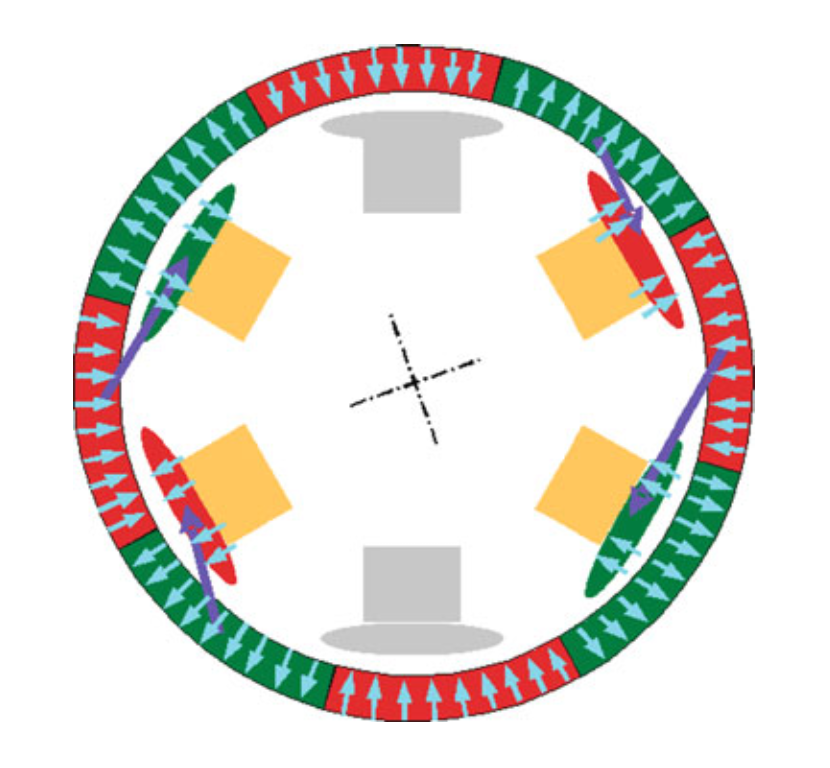
\includegraphics[width=0.45\linewidth]{images/AufbauBLDC} \label{figAufbauBLDC} 	}
\subfigure[Sinstr][Sinusstrom mit PWM-Spannung \cite{InTech_PWM}]{ 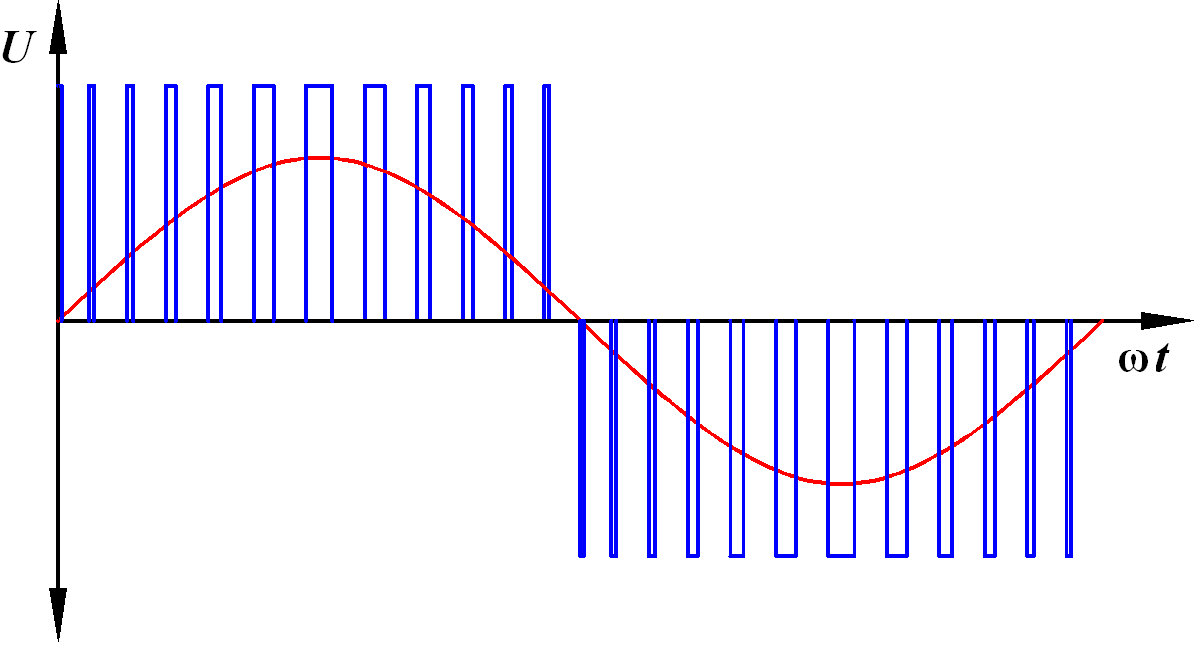
\includegraphics[width=0.5\linewidth]{images/StromBLDC} \label{figSinusstromPWM}}
\caption[BLDC Motor]{Aufbau BLDC und PWM-Ansteuerung}
\label{fig:BLDC}
\end{figure}

Angesteuert wird jede Phase über eine Halbbrücke. Die FOC-Regelungsweise (siehe Kapitel \ref{tGl_FOC}), setzt einen sinusförmigen Strom auf jeder Phase voraus, dies jeweils 120\(^\circ\) Phasenverschoben. \todo{ausschreiben od mit Zeichen? 120\(^\circ\) od 120 Grad?} Realisiert wird dies mittels PWM-Ansteuerung der Halbbrücken. Da der Strom bei einer L-Last das Integral der Spannung ist, lässt sich ein quasi-sinusförmiger Strom generieren. Dargestellt ist dies in der Abbildung \ref{figSinusstromPWM}.

\begin{center}
\begin{tabular}{|c|c|}
\hline 
\rule[-1ex]{0pt}{2.5ex}  BLDC Motor & Werte  \\ 
\hline 
\rule[-1ex]{0pt}{2.5ex} Idle Current & 1.2A \\ 
\hline 
\rule[-1ex]{0pt}{2.5ex} Max. Current & 50A \\ 
\hline
\rule[-1ex]{0pt}{2.5ex} Input Volt. & 2..10 x 3.6 Lipo (25.2V) \\ 
\hline
\rule[-1ex]{0pt}{2.5ex} Max. Output & 1815W \\ 
\hline
\rule[-1ex]{0pt}{2.5ex} Max. Pull & 6700g \\ 
\hline
\rule[-1ex]{0pt}{2.5ex} Rated Curren & 42.5A \\ 
\hline
\rule[-1ex]{0pt}{2.5ex} Motor Weight & 460g \\ 
\hline
\rule[-1ex]{0pt}{2.5ex} Shaft & 8mm \\ 
\hline
\rule[-1ex]{0pt}{2.5ex} Motor dimension & \O 50 x 65mm \\ 
\hline
\rule[-1ex]{0pt}{2.5ex} Internal Resistance & 0.0361$\Omega$ \\ 
\hline	
\end{tabular} 
\captionof{table}{BLDC Daten}
\label{tabBLDCdaten}
\end{center}

\todo{e-Deutsch uebersetzung und Formatierung usw}
\todo{ev in Anhang??}
\todo{\cite{ElAntriebe_Babiel} und korrekt zitieren...}


\subsection{FOC}
\label{tGl_FOC}
Einstieg...\todo{Einstieg}\\
\todo{LEserführung, Metaebene!}\\
\todo{Bilder und Quellen}
Das Prinzip der Transformationen:
Ein kompliziertes Problem wird in ein anderes Koordinatensystem transformiert. Das transformierte Problem ist dort viel einfacher zu lösen, es ist also ein einfacheres Problem. Die leicht gefundene Lösung wird rücktransformiert, wodurch die Lösung des komplizierten Problems erhalten wird. Ein mögliches Beispiel dafür ist die Laplace-Transformierung von Differentialgleichungen. 
\\
In unserem Beispiel ist das Problem die Ansteuerung des Motors. Mit der Clarke-Transformation wird in ein statorfestes Koordinatensystem gewechselt, mit der anschliessenden Park-Transformation in ein rotorfestes. Das Problem ist nun linear und mit einem einfachen PI (oder PID) Regler lösbar. \\
Anschliessend wird die gefundene Lösung zurücktransformiert. Dabei kann die komplette Rücktransformation (inverse Park- und inverse Clarke Transformation) ausgeführt und anschliessend der Motor über eine PWM angesteuert werden, oder aber es wird nur bis ins statorfeste Koordinatensystem rücktransformiert, (inverse Park Transformation) dann wird der Motor über eine Raumvektor-PWM (SVPWM) angesteuert.


\subsubsection{Clarke- und Park-Transformation}
\todo{Leserführung}
\todo{ev. subsections nummeriert?!}
\todo{Bmk dass nicht nur für I sondern auch für U usw... und I nur exemplarisch gilt}
Im Folgenden wird die Clarke- und die Park-Transformation erklärt. \todo{......ev. mgl, die Abb. bereits hierhin zu nehmen?}
\begin{figure} [H]
	\centering
	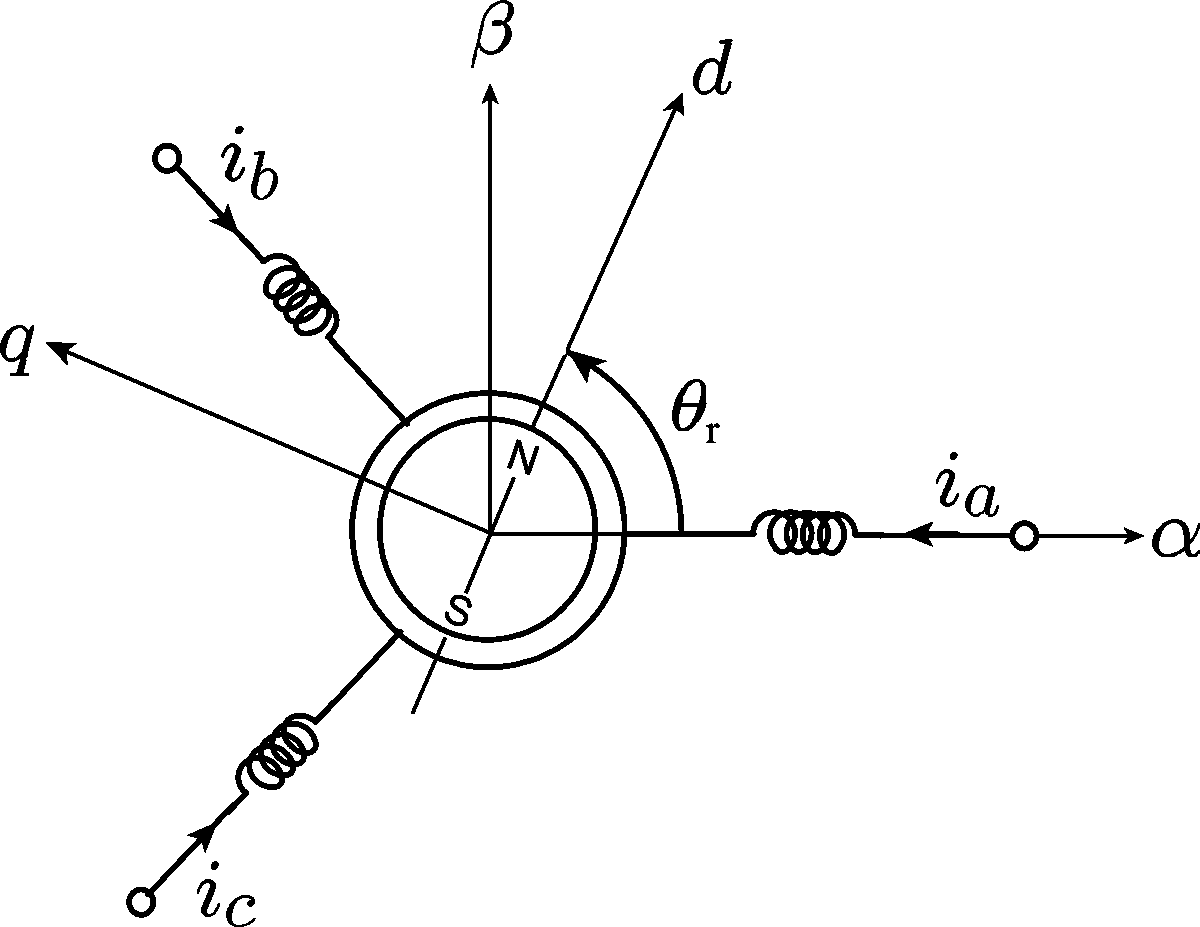
\includegraphics[width=1\linewidth]{images/trafo_schematicPMSM}
	\caption{Schematische Darstellung einer PMSM mit den drei Koordinatensystemen }
	\label{fig:trafoschematicpmsm}
\end{figure}

\subsubsection*{Clarke-Transformation}
\todo{weitere unterstrukturierung mgl?}
Die Clarke-Transformation wechselt die mehr- bzw. dreiphasigen Grössen (z.B. Phasenströme) in ein statorfestes Bezugssystem. Das kartesische Koordinatensystem ist in der komplexen Ebene. Die drei Phasenströme I$_{a}$, I$_{b}$ und I$_{c}$ werden auf zwei komplexwertige Ströme I$_{\alpha}$ und I$_{\beta}$ abgebildet. Dargestellt ist die Transformation in der Abbildung \ref{fig:trafoschematicpmsm}.
%Die Transformation kann geometrisch hergeleitet werden. (xxx…)
Die mathematische Formulierung lautet:
\begin{equation}\label{ClarkeTrafo}
\left[
\begin{array}{c}
I_\alpha \\ 
I_\beta
\end{array} 
\right]
= \frac{2}{3}
\left[
\begin{array}{ccc}
1 & -\frac{1}{2} & -\frac 12 \\ 
0 & \frac{\sqrt{3}}{2} & -\frac{\sqrt{3}}{2}
\end{array} 
\right] 
\left[
\begin{array}{c}
I_A \\ 
I_B \\
I_C
\end{array} 
\right]
\end{equation}
\todo{Abstände zwischen den Zeilen der Matrix?! ... schönere Darstellung gewünscht; Entscheid ob Multiplikationspunkt cdot dazwischen}
Die inverse Clarke-Transformation wird entsprechend durch folgende Gleichung beschrieben:
\begin{equation}\label{invClarkeTrafo}
\left[
\begin{array}{c}
I_A \\ 
I_B \\
I_C
\end{array} 
\right]
= 
\left[
\begin{array}{cc}
1 & 0 \\
-\frac{1}{2} & \frac{\sqrt{3}}{2} \\
-\frac 12  & -\frac{\sqrt{3}}{2}
\end{array} 
\right] 
\left[
\begin{array}{c}
I_\alpha \\ 
I_\beta
\end{array} 
\right]
\end{equation}


\subsubsection*{Park-Transformation}
Die Park-Transformation transformiert die Grössen I$_{\alpha}$ und I$_{\beta}$ in ein rotorfestes Bezugssystem. Dieses neue kartesische Koordinatensystem besteht aus zwei Achsen, und von aussen gesehen (ruhendes Bezugssystem) rotiert es mit der gleichen Winkelgeschwindigkeit wie der Rotor. Eine Achse wird als d-Achse (direct axis) bezeichnet, die andere als q-Achse (quadrature axis). Die d-Achse beschreibt die magnetische Flussdichte des Rotors, die q-Achse das Drehmoment des Rotors. \\
Ausgehend vom statorfesten Bezugssystem benötigt es nur noch eine Rotation, um die Grössen in das rotorfeste Bezugssystem zu transformieren. Mathematisch gesehen geschieht die Transformation also über eine Drehmatrix, dargestellt ist die Transformation in der Gleichung \ref{ParkTrafo}. 
\begin{equation}\label{ParkTrafo}
\left[
\begin{array}{c}
I_d \\ 
I_q
\end{array} 
\right]
= 
\left[
\begin{array}{cc}
\cos (\theta) & \sin(\theta) \\
-\sin(\theta)  & \cos(\theta)
\end{array} 
\right] 
\left[
\begin{array}{c}
I_\alpha \\ 
I_\beta
\end{array} 
\right]
\end{equation}

Die inverse Park-Transformation wird entsprechend durch folgende Gleichung beschrieben:
\begin{equation}\label{invParkTrafo}
\left[
\begin{array}{c}	
I_\alpha \\ 
I_\beta
\end{array} 
\right]
= 
\left[
\begin{array}{cc}
\cos (\theta) & -\sin(\theta) \\
\sin(\theta)  & \cos(\theta)
\end{array} 
\right] 
\left[
\begin{array}{c}
I_d \\ 
I_q
\end{array} 
\right]
\end{equation}

\subsubsection*{d/q-Transformation} 
Die Clarke- und Park-Transformation kann auch in einem Schritt durchgeführt werden, je nach Quelle wird diese dann auch Park-Transformation oder d/q-Transformation genannt. [xxx Quelle!] \todo{Quelle}
Die mathematische Formulierung lautet:
\begin{equation}\label{dqTrafo}
\left[
\begin{array}{c}
I_d \\ 
I_q
\end{array} 
\right]
= \frac{2}{3}
\left[
\begin{array}{ccc}
\cos (\theta) & \cos (\theta-\frac{2\pi}{3} & \cos (\theta-\frac{4\pi}{3} \\ 
-\sin (\theta) & -\sin (\theta-\frac{2\pi}{3} & -\sin (\theta-\frac{4\pi}{3}
\end{array} 
\right] 
\left[
\begin{array}{c}
I_A \\ 
I_B \\
I_C
\end{array} 
\right]
\end{equation}

Die inverse d/q-Transformation lautet:
\begin{equation}\label{invdqTrafo}
\left[
\begin{array}{c}
I_A \\ 
I_B \\
I_C
\end{array} 
\right]
=
\left[
\begin{array}{cc}
\cos (\theta) & -\sin (\theta) \\
\cos (\theta-\frac{2\pi}{3} & -\sin (\theta-\frac{2\pi}{3} \\
\cos (\theta-\frac{4\pi}{3} & -\sin (\theta-\frac{4\pi}{3} 
\end{array} 
\right] 
\left[
\begin{array}{c}
I_d \\ 
I_q
\end{array} 
\right]
\end{equation}


\subsubsection{PI-Regler}
Der PI-Regler ist ein Regler mit einem Proportional- (P) und einem Integral- (I) Glied. Dies sind elementare Glieder der Regelungstechnik. Das P-Glied entspricht einer Multiplikation des Eingangs mit einer zeitunabhängigen Konstanten, das P-Glied einer Integration des Eingangs. 
\\
Die Regelung mit einem PI-Regler geschieht im rotorfesten Bezugssystem, Gegenstand der Regelung sind die Flussdichte des Motors (d-Komponente) und das Drehmoment (q-Komponente). Bei einem permanenterregten Motor ist diese Regelung vereinfacht. In der Abb.\ref{fig:trafoschematicpmsm} ist ersichtlich, dass die d-Achse in Richtung des Permanentmagneten zeigt. Das grösste resultierende Moment wird erreicht, wenn die resultierende Flussdichte im Stator um 90\(^\circ\) zur zeitlich konstanten Flussdichte des Rotors verschoben ist. Dies zeigt also genau in Richtung der q-Achse. Die resultierende Flussdichte liegt also auf der q-Achse und hat deshalb keinen d-Anteil. Der Sollwert der d-Komponente wird also null. Das Drehmoment kann somit direkt über die q-Komponente geregelt werden. 

\todo{Ev. Begründung warum PI Regler, ohne D, Iteil grösser… träges system, d für schenlle änderungen}

\subsubsection{Nonlinear Observer}
Die Park-Transformation benötigt die momentane Lage des Rotors. Da der vorgegebene Motor nicht über integrierte Sensoren (wie beispielsweise Hall-Sonden) verfügt, die Ansteuerung also sensorlos erfolgt, muss der Winkel der Rotorlage auf einem anderen Weg herausgefunden werden. Dazu gibt es verschiedene Varianten. 
Ev. Tabelle mit Variante, Pro, Contra; Erläuerungen \todo{Tabelle od Ausformulierung der Gründe für diese Variante}
Im Team wurde entschieden, die Winkelschätzung über einen nichtlinearen Beobachter, nonlinear observer genannt, vorzunehmen. (Formulierung! Und Begründung…) Dazu wird ein mathematisches Modell des Motors erstellt. Zudem werden die Phasenströme gemessen. Mit diesen Informationen wird eine Simulation des Motors durchgeführt, und aufgrund der aktuellen Parameter wird die Position ermittelt. Dies funktioniert, da aufgrund der Phasenströme auf die Lage des Motors rückgeschlossen werden kann. Beschrieben wird dieses Verfahren in xxx [Quelle IEEE-Paper].
\todo{Quelle nonlinear Observer}

\subsection{H-Brücke}
Wie in Abbildung \ref{fig:BLDC} zu sehen, muss eine sinusförmige Spannung am Motor anliegen. Die FOC-Berechnungen aus Kapitel \ref{tGl_FOC} ergeben zeitdiskrete Spannungswerte. Diese werden mit der Raumvektor-PWM Methode in PWM Signale umgewandelt welche mit der H-Brücke ausgegeben werden. Die H-Brücke besteht aus drei Halbbrücken mit je zwei N-Kanal MOSFETs. 
\begin{center}
	\begin{circuitikz}[scale=2]
		\draw[color=black]
		% Fet, Fet and Resistor
		(0,1) node[nigfete] (nmos1) {}
		(0,0) node[nigfete] (nmos2) {}
		(nmos1.S) to (nmos2.D)
		(nmos2.S) to [R, l_=$R_{sense1}$] (0,-1.5) -- (1,-1.5)
		(nmos1.D) |- (1,1.5)
		% Fet, Fet and Resistor
		(2,1) node[nigfete] (nmos3) {}
		(2,0) node[nigfete] (nmos4) {}
		(nmos3.S) to (nmos4.D)
		(nmos4.S) to [R, l_=$R_{sense2}$] (2,-1.5) -- (2,-1.5)
		(nmos3.D) |- (1,1.5)
		% Fet, Fet
		(4,1) node[nigfete] (nmos5) {}
		(4,0) node[nigfete] (nmos6) {}
		(nmos5.S) to (nmos6.D)
		(nmos6.S) |- (1,-1.5)
		(nmos6.D) |- (1,1.5)

		% ground
		(2,-1.5) node[ground]{}
		% supply
		(2,1.5) to [short,-o] (2,2) node[right]{$V_{BAT}$}
		% gates
		(nmos1.G) to [short,-o] ++(-0.1,0) node[left]{$AH$}
		(nmos2.G) to [short,-o] ++(-0.1,0) node[left]{$AL$}
		(nmos3.G) to [short,-o] ++(-0.1,0) node[left]{$BH$}
		(nmos4.G) to [short,-o] ++(-0.1,0) node[left]{$BL$}
		(nmos5.G) to [short,-o] ++(-0.1,0) node[left]{$CH$}
		(nmos6.G) to [short,-o] ++(-0.1,0) node[left]{$CL$}
		%outputs
		(nmos1.S) ++(0,-0.1) to [short,-o] ++(0.5,0) node[right]{$A$}
		(nmos3.S) ++(0,-0.1) to [short,-o] ++(0.5,0) node[right]{$B$}
		(nmos5.S) ++(0,-0.1) to [short,-o] ++(0.5,0) node[right]{$C$}
		;
		% junctions
		\fill (2,-1.5) circle(1pt);
		\fill (2,1.5) circle(1pt);
		\fill (nmos1.S) ++(0,-0.1) circle(1pt);
		\fill (nmos3.S) ++(0,-0.1) circle(1pt);
		\fill (nmos5.S) ++(0,-0.1) circle(1pt);
	\end{circuitikz}
	\captionof{figure}{H-Brücke zur Motoransteuerung}
	\label{fig:hbridge}
\end{center}

Mit den sogenannten High-Side MOSFETs kann jede Phase einzeln auf die Batteriespannung geschaltet werden. Die Low-Side FETs arbeiten symmetrisch dazu und können die Phase auf Batteriemasse schalten. Durch die berechneten PWM kann so ein dreiphasiger Sinus approximiert werden. 

Damit nicht gleichzeitig die High- und Low-Side FETs einer Phase eingeschaltet sind, was zu einem Kurzschluss führen würde, ist im Treiber IC eine totzeit Schaltung eingebaut. Wird der eine FET ausgeschaltet sind für eine kurze Zeit beide ausgeschaltet bevor der nächste eingeschaltet werden kann. Dieses Verfahren wird Dedatime genannt.

\label{tGl_HBrugg}
\subsection{Funkübertragung}
\label{tGl_RF}
